\documentclass[journal]{IEEEtran}

\usepackage{amsmath,amssymb}
\usepackage{graphicx}
\usepackage{booktabs}
\usepackage{array}
\usepackage{siunitx}
\usepackage{url}
\usepackage{xcolor}
\usepackage{tikz}
\usetikzlibrary{arrows.meta,positioning,calc}

\sisetup{
  detect-all,
  group-digits=false,
  exponent-product=\times
}

\newcommand{\R}{\mathbb{R}}
\newcommand{\rank}{\operatorname{rank}}
\newcommand{\range}{\operatorname{range}}
\newcommand{\nullsp}{\operatorname{null}}
\newcommand{\pinv}{\dagger}
\newcommand{\PR}{P_{\mathrm{R}}}
\newcommand{\PZ}{P_{0}}
\newcommand{\RelMeasErr}{\mathrm{RelMeasErr}}
\newcommand{\Audit}{\Pi_y^\lambda}
\newcommand{\Blambda}{B_\lambda}

\definecolor{RangeBlue}{HTML}{2F6FED}
\definecolor{NullOrange}{HTML}{E28B2C}
\definecolor{AuditBg}{HTML}{FAFAF8}

\begin{document}

\title{Measurement Auditing for Learned Ghost Imaging: Certificates, Limits, and Prior-Supplied Content}

\author{[Authors omitted for review]}

\markboth{MEASUREMENT AUDITING FOR LEARNED GHOST IMAGING}{MEASUREMENT AUDITING FOR LEARNED GHOST IMAGING}

\maketitle

\begin{abstract}
Learned ghost-imaging reconstructions can be visually plausible while still leaving unclear which image content is supported by the recorded bucket measurements and which content is supplied by the prior.  This paper develops a range-null view of this question.  For a sensing matrix $A\in\R^{m\times n}$, $m\ll n$, the row-space projector $\PR=A^\pinv A$ and null-space projector $\PZ=I-A^\pinv A$ give the unique orthogonal decomposition $x=\PR x+\PZ x$.  The measurement record constrains only $\PR x$; $\PZ x$ is invisible to $A$.  This single geometric fact separates measurement accountability from image quality, and it also exposes a limit: consistency with the bucket measurements is not correctness of the unmeasured image content.  We then attach to any reconstructor a test-time measurement audit,
$\Audit(v)=v-\Blambda(Av-y)$ with $\Blambda=A^\top(AA^\top+\lambda I)^{-1}$, and prove that its residual contracts by the singular-mode factor $\lambda/(\lambda+\sigma_i^2)$.  Experiments show that the same audit reduces measurement residuals for BP, Tikhonov, CS-TV, and learned outputs while moving PSNR only slightly for trained outputs.  A GAN branch is used only as a representative generative prior: it illustrates controlled prior-supplied detail under the same audit, not a claim of state-of-the-art image quality or superiority over diffusion models.
\end{abstract}

\begin{IEEEkeywords}
Ghost imaging, inverse problems, measurement consistency, null space, range space, learned reconstruction, GAN, certification.
\end{IEEEkeywords}

\section{Introduction}

Low-rate ghost imaging and single-pixel imaging acquire a small number of bucket measurements from structured illumination patterns [CITE].  At sampling rates such as 5--10\%, the inverse problem is deeply underdetermined: many images agree with the same measurement vector.  Modern learned priors, including adversarial and other generative priors, can fill the missing visual structure and produce reconstructions that look plausible.  The scientific question is therefore not only whether the image is visually good.  It is also: which part of the image is supported by the recorded measurement, and which part was supplied by the prior?

Standard image metrics do not answer this question.  PSNR and SSIM require a ground-truth image, which is unavailable in deployment, and they mix together measured and unmeasured error.  A high PSNR image can still have a measurement residual, while a measurement-consistent image can still be semantically wrong in its unmeasured component.  A useful reconstruction pipeline for undersampled imaging should therefore report a ground-truth-free measurement-accountability certificate in addition to image-quality metrics.

This work takes a deliberately geometric route.  Let $A\in\R^{m\times n}$, $m\ll n$, be the ghost-imaging measurement operator.  The Moore--Penrose row-space projector $\PR=A^\pinv A$ and null-space projector $\PZ=I-A^\pinv A$ split every image into measured and unmeasured components.  This decomposition is not a modeling assumption; it is the linear algebra of the measurement operator.  The row component $\PR x$ is the part seen by the bucket measurements, while $\PZ x$ is exactly invisible to them.

The paper's contributions are:

\begin{itemize}
    \item We use the range-null decomposition to give a strict separability statement for measurement accountability and prior-supplied image content.  The measurement $y=Ax$ constrains $A(\PR x)$ and never constrains $A(\PZ x)$.
    \item We define a plug-in test-time audit $\Audit$ that can be applied after any reconstructor.  We prove its singular-mode residual contraction exactly and report the corresponding measurement certificate.
    \item We state the boundary of this certificate.  The audit certifies agreement with the recorded measurements; it does not certify that the unmeasured component is true.  We empirically map this boundary through feasible hallucinations, operator-drift and wrong-measurement probes, and posterior-calibration diagnostics.
    \item We use a GAN branch as a representative generative prior under this audit.  The GAN is not the novelty claim and is not presented as a state-of-the-art benchmark result or as a comparison against diffusion models.
\end{itemize}

\begin{figure*}[t]
    \centering
    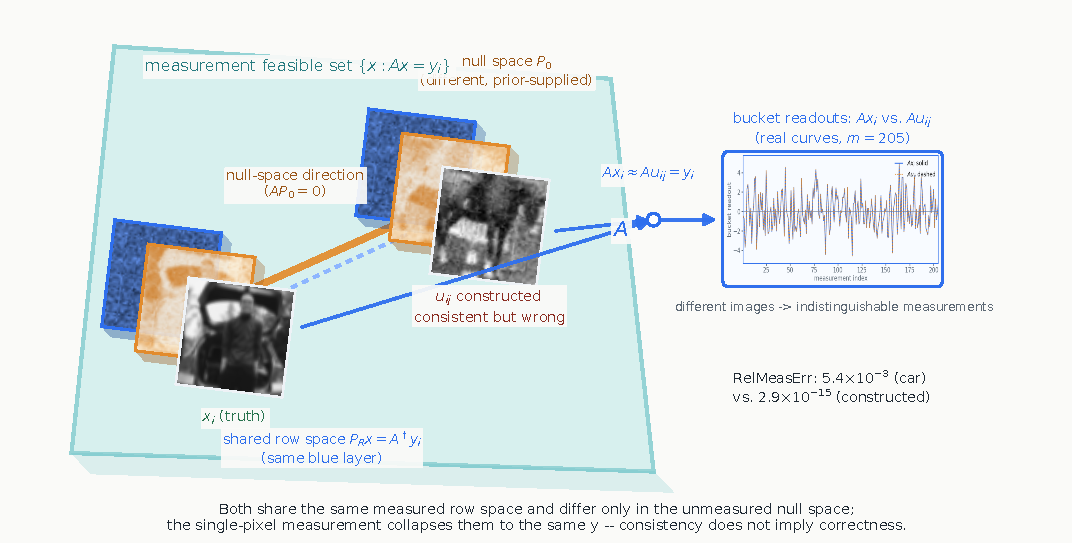
\includegraphics[width=\textwidth]{figures/figure1_feasible_geometry.pdf}
    \caption{Range-null decomposition and the ghost-imaging bucket readout for
    the Rad-5 pair $i=1789$, $j=935$.  Each image card is drawn as a real
    three-layer stack: the shared blue row-space layer is the measurement-locked
    skeleton $P_Rx=A^\dagger y_i$, the orange layer is the null-space component,
    and the top layer is the displayed image.  The car truth $x_i$ uses
    $P_0x_i$, whereas the constructed image
    $u_{ij}=x_j-A^\dagger(Ax_j-y_i)$ uses the horse donor's $P_0x_j$; hence the
    two cards share the measured row space and differ only in the unmeasured
    null space.  Both are sent through the same single-pixel measurement
    operator, and the right panel plots the real bucket readout vector
    $y_i=y[1789]$ ($m=205$), not a schematic.  The car truth has the
    noisy-record residual $\RelMeasErr(x_i,y_i)=\num{5.36e-3}$, while the
    constructed image satisfies
    $\RelMeasErr(u_{ij},y_i)=\num{2.93e-15}$.  The displayed $u_{ij}$ is clipped
    for visualization and is constructed, measurement-consistent, semantically
    wrong, and not a natural image.  Thus measurement-consistent $\ne$ correct
    $\ne$ natural.}
    \label{fig:pipeline-range-null}
\end{figure*}

All numerical values reported in the tables are from the experiments described
in this manuscript.

\section{Problem Setup and Range-Null Decomposition}

\subsection{Forward Model}

We consider the standard linear ghost-imaging model
\begin{equation}
    y = Ax+\varepsilon,
    \label{eq:forward}
\end{equation}
where $x\in\R^n$ is the vectorized image, $y\in\R^m$ is the bucket-measurement vector, $A\in\R^{m\times n}$ is the measurement matrix, $m\ll n$, and $\varepsilon$ is measurement noise.  Let the compact singular value decomposition of $A$ be
\begin{equation}
    A = U_r \Sigma_r V_r^\top,
    \label{eq:compact-svd}
\end{equation}
where $r=\rank(A)$, $U_r\in\R^{m\times r}$ and $V_r\in\R^{n\times r}$ have orthonormal columns, and $\Sigma_r=\operatorname{diag}(\sigma_1,\ldots,\sigma_r)$ with $\sigma_i>0$.

The Moore--Penrose pseudoinverse is
\begin{equation}
    A^\pinv = V_r \Sigma_r^{-1} U_r^\top.
\end{equation}
Therefore
\begin{equation}
    \PR = A^\pinv A
        = V_r \Sigma_r^{-1} U_r^\top U_r \Sigma_r V_r^\top
        = V_r V_r^\top,
    \label{eq:pr-vv}
\end{equation}
and
\begin{equation}
    \PZ = I-\PR = I-V_rV_r^\top.
    \label{eq:p0-def}
\end{equation}
Since $V_r^\top V_r=I_r$, we have
\begin{align}
    \PR^2 &= (V_rV_r^\top)(V_rV_r^\top)
           =V_r(V_r^\top V_r)V_r^\top
           =V_rV_r^\top=\PR,\\
    \PR^\top &= \PR,
\end{align}
so $\PR$ is an orthogonal projector.  The same identities give
\begin{align}
    \PZ^2 &= (I-\PR)^2=I-2\PR+\PR^2=I-\PR=\PZ,\\
    \PZ^\top &= \PZ.
\end{align}
Moreover,
\begin{equation}
    \PR\PZ=\PR(I-\PR)=\PR-\PR^2=0.
\end{equation}
Thus, for every image $x$,
\begin{equation}
    x = \PR x+\PZ x,
    \label{eq:orth-decomp}
\end{equation}
and
\begin{equation}
    \langle \PR x,\PZ x\rangle
    = x^\top \PR^\top\PZ x
    = x^\top \PR\PZ x
    =0.
    \label{eq:orthogonality}
\end{equation}

\textit{Plain-language interpretation:} every image splits uniquely into a measured row-space part and an unmeasured null-space part, and the two parts do not overlap in energy.

\subsection{Measurements Constrain Only the Row Space}

We now derive the central separability statement.  First,
\begin{align}
    A\PZ
    &= A(I-A^\pinv A) \\
    &= A-AA^\pinv A.
\end{align}
The Moore--Penrose identities give $AA^\pinv A=A$, so
\begin{equation}
    A\PZ=0.
    \label{eq:ap0-zero}
\end{equation}
Similarly,
\begin{align}
    A\PR
    &= A(A^\pinv A)\\
    &= (AA^\pinv A)\\
    &= A.
    \label{eq:apr-a}
\end{align}
Combining \eqref{eq:orth-decomp}, \eqref{eq:ap0-zero}, and \eqref{eq:apr-a},
\begin{align}
    Ax
    &= A(\PR x+\PZ x)\\
    &= A\PR x + A\PZ x\\
    &= A\PR x.
    \label{eq:y-only-range}
\end{align}
Therefore the measurement record is a function only of $\PR x$.

In the noiseless case, if $Ax=y$, then
\begin{equation}
    \PR x = A^\pinv A x = A^\pinv y.
    \label{eq:unique-row}
\end{equation}
Thus every feasible image with the same measurement $y$ has the same row-space component $A^\pinv y$.  Conversely, for any $z_0\in\nullsp(A)$,
\begin{align}
    A(A^\pinv y+z_0)
    &= AA^\pinv y + Az_0.
\end{align}
When $y\in\range(A)$, $AA^\pinv y=y$, and $Az_0=0$, so
\begin{equation}
    A(A^\pinv y+z_0)=y.
\end{equation}
The set of noiseless feasible images is therefore
\begin{equation}
    \{x:Ax=y\} = A^\pinv y+\nullsp(A).
    \label{eq:affine-feasible}
\end{equation}
With noise, $A^\pinv y$ is the least-squares row-space estimate induced by the recorded measurement, while the null component remains unobserved by $A$.

\textit{Plain-language interpretation:} the bucket measurements determine the measured component and say nothing about the null-space content; the underdetermined part is not a weakness of a particular algorithm, but a geometric fact about $A$.

\section{Measurement Audit and Its Contraction Certificate}
\label{sec:audit}

\subsection{A Plug-In Audit}

Let $v\in\R^n$ be the output of any reconstructor: a backprojection, a variational solver, a neural network, or a generative model.  Define
\begin{equation}
    \Blambda = A^\top(AA^\top+\lambda I)^{-1},\qquad \lambda>0,
    \label{eq:blambda}
\end{equation}
and the test-time audit
\begin{equation}
    \Audit(v)=v-\Blambda(Av-y).
    \label{eq:audit}
\end{equation}
The audit uses only $A$, $y$, and the candidate output $v$; it does not retrain the reconstructor.

The update direction $\Blambda(Av-y)$ lies in $\range(A^\top)$, which is the row space of $A$.  Hence
\begin{equation}
    \PZ\Blambda(Av-y)=0,
\end{equation}
and therefore
\begin{equation}
    \PZ\Audit(v)=\PZ v.
    \label{eq:audit-null-unchanged}
\end{equation}
The audit changes only the measurement-visible component.

\textit{Plain-language interpretation:} the audit can repair bucket consistency, but it does not rewrite the prior-supplied null-space image content.

\begin{figure*}[t]
    \centering
    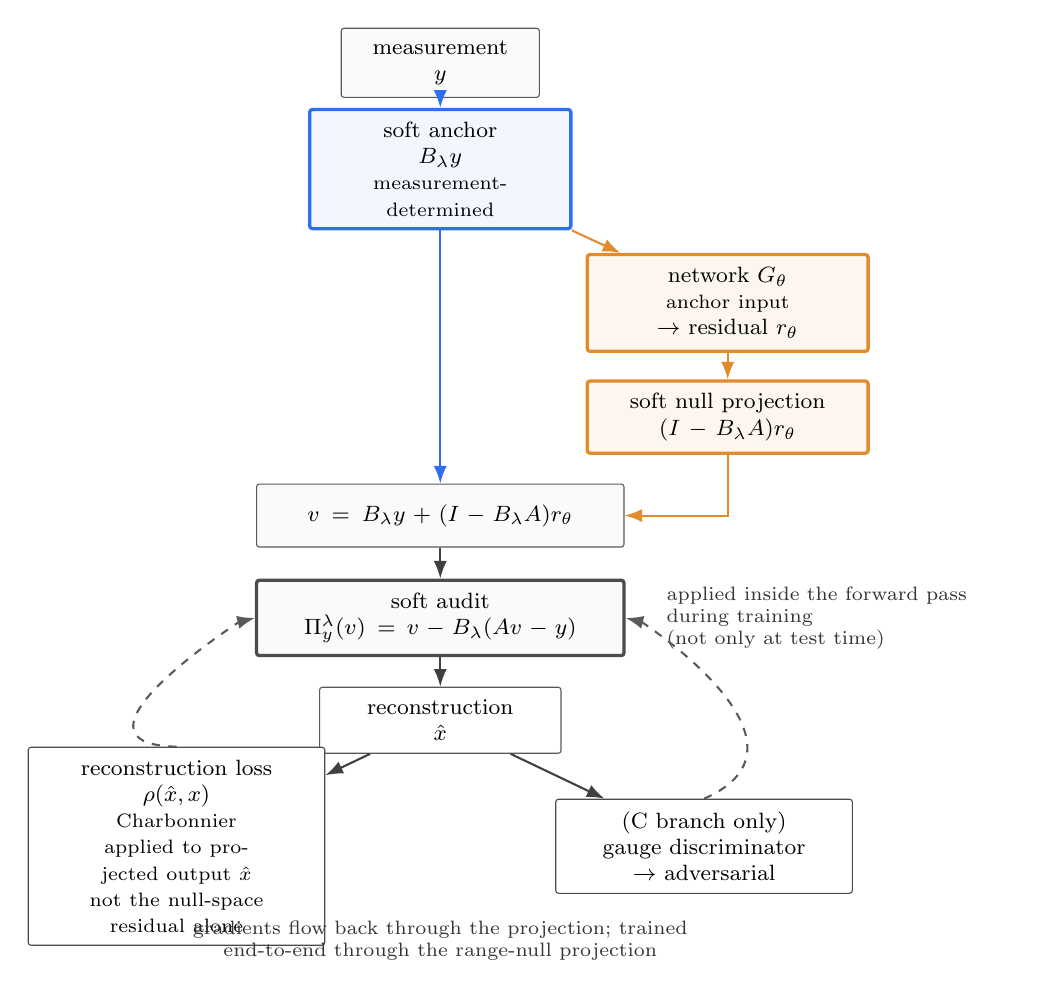
\begin{tikzpicture}[
        >=Latex,
        font=\footnotesize,
        box/.style={
            draw=black!65,
            rounded corners=1pt,
            align=center,
            inner sep=4.5pt,
            minimum height=0.80cm,
            fill=white
        },
        rangebox/.style={
            box,
            draw=RangeBlue,
            very thick,
            fill=RangeBlue!6
        },
        nullbox/.style={
            box,
            draw=NullOrange,
            very thick,
            fill=NullOrange!8
        },
        auditbox/.style={
            box,
            draw=black!70,
            very thick,
            fill=AuditBg
        },
        lossbox/.style={
            box,
            draw=black!70,
            fill=white
        },
        note/.style={
            align=left,
            font=\scriptsize,
            text=black!80
        },
        arrow/.style={->, line width=0.75pt, draw=black!75},
        bluearrow/.style={arrow, draw=RangeBlue},
        orangearrow/.style={arrow, draw=NullOrange},
        backarrow/.style={->, dashed, line width=0.75pt, draw=black!65}
    ]
        \node[box, fill=AuditBg, text width=2.2cm] (y) at (0,0)
            {measurement\\$y$};
        \node[rangebox, text width=3.0cm] (anchor) at (0,-1.35)
            {soft anchor\\$\Blambda y$\\{\scriptsize measurement-determined}};

        \node[nullbox, text width=3.25cm] (net) at (3.65,-3.05)
            {network $G_\theta$\\{\scriptsize anchor input}\\$\to$ residual $r_\theta$};
        \node[nullbox, text width=3.25cm] (pnull) at (3.65,-4.50)
            {soft null projection\\$(I-\Blambda A)r_\theta$};

        \node[box, fill=AuditBg, text width=4.35cm] (v) at (0,-5.75)
            {$v=\Blambda y+(I-\Blambda A)r_\theta$};
        \node[auditbox, text width=4.35cm] (audit) at (0,-7.05)
            {soft audit\\$\Audit(v)=v-\Blambda(Av-y)$};
        \node[note, text width=4.4cm, anchor=west] (auditnote) at (2.75,-7.05)
            {applied inside the forward pass during training\\(not only at test time)};

        \node[box, fill=white, text width=2.75cm] (xhat) at (0,-8.35)
            {reconstruction\\$\hat{x}$};
        \node[lossbox, text width=3.45cm] (rec) at (-3.35,-9.95)
            {reconstruction loss\\$\rho(\hat{x},x)$\\{\scriptsize Charbonnier}\\{\scriptsize applied to projected output $\hat{x}$}\\{\scriptsize not the null-space residual alone}};
        \node[lossbox, text width=3.45cm] (adv) at (3.35,-9.95)
            {(C branch only)\\gauge discriminator\\$\to$ adversarial};
        \node[note, align=center, text width=7.2cm] (gradnote) at (0,-11.15)
            {gradients flow back through the projection; trained end-to-end through the range-null projection};

        \draw[bluearrow] (y) -- (anchor);
        \draw[bluearrow] (anchor) -- (v);
        \draw[orangearrow] (anchor) -- (net);
        \draw[orangearrow] (net) -- (pnull);
        \draw[orangearrow] (pnull) |- (v);
        \draw[arrow] (v) -- (audit);
        \draw[arrow] (audit) -- (xhat);
        \draw[arrow] (xhat) -- (rec);
        \draw[arrow] (xhat) -- (adv);
        \draw[backarrow] (rec.north) .. controls (-4.95,-8.65) and (-2.55,-7.10) .. (audit.west);
        \draw[backarrow] (adv.north) .. controls (4.95,-8.65) and (2.55,-7.10) .. (audit.east);
    \end{tikzpicture}
    \caption{Simplified training pipeline.  The measurement gives a soft anchor
    $\Blambda y$, the network supplies a null-space completion through the
    soft null projection $I-\Blambda A$, and the soft audit $\Audit$ is applied
    inside the training forward pass before the reconstruction loss.  The
    reconstruction loss is applied to the projected full image $\hat{x}$, not
    to the null-space residual alone; thus gradients pass through the
    range-null projection while the C branch adds a gauge adversarial term.
    The blue path marks measurement-determined row-space content and the orange
    path marks prior-supplied null-space content.  The exact geometric
    decomposition uses $\PR=A^\dagger A$ and $\PZ=I-A^\dagger A$, whereas the
    implementation uses the noise-aware soft operators
    $\Blambda=A^\top(AA^\top+\lambda I)^{-1}$ and $\Audit$ with $\lambda>0$
    (the code uses $\lambda=0.001$).  For clarity this shows the conceptual
    data flow; the full implementation is a two-stage reconstructor with a
    refinement stage and two soft-audit applications, simplified here as one
    audit block, and uses the soft (ridge) projection $\Blambda$ with
    $\lambda>0$, which approaches the exact projection as $\lambda\to0$.}
    \label{fig:training-architecture}
\end{figure*}

\subsection{Residual Contraction}

Let
\begin{equation}
    r(v)=Av-y
\end{equation}
be the measurement residual before audit.  Applying $A$ to \eqref{eq:audit} gives
\begin{align}
    A\Audit(v)-y
    &= A\left(v-A^\top(AA^\top+\lambda I)^{-1}(Av-y)\right)-y\\
    &= Av-y-AA^\top(AA^\top+\lambda I)^{-1}(Av-y)\\
    &= \left[I-AA^\top(AA^\top+\lambda I)^{-1}\right]r(v).
    \label{eq:resid-step1}
\end{align}
Now use
\begin{align}
    AA^\top(AA^\top+\lambda I)^{-1}
    &= \left[(AA^\top+\lambda I)-\lambda I\right](AA^\top+\lambda I)^{-1}\\
    &= I-\lambda(AA^\top+\lambda I)^{-1}.
    \label{eq:matrix-identity}
\end{align}
Substituting \eqref{eq:matrix-identity} into \eqref{eq:resid-step1},
\begin{align}
    A\Audit(v)-y
    &= \left[I-\left(I-\lambda(AA^\top+\lambda I)^{-1}\right)\right]r(v)\\
    &= \lambda(AA^\top+\lambda I)^{-1}(Av-y).
    \label{eq:contraction-main}
\end{align}

To see the mode-wise certificate, write
\begin{equation}
    AA^\top = U_r\Sigma_r^2 U_r^\top
\end{equation}
on the nonzero left singular subspace.  If $r(v)=\sum_{i=1}^r \alpha_i u_i$ in that subspace, then
\begin{align}
    A\Audit(v)-y
    &= \lambda U_r(\Sigma_r^2+\lambda I)^{-1}U_r^\top
       \sum_{i=1}^r \alpha_i u_i\\
    &= \sum_{i=1}^r
       \frac{\lambda}{\sigma_i^2+\lambda}\alpha_i u_i.
    \label{eq:mode-contraction}
\end{align}
Thus each measured singular mode contracts by
\begin{equation}
    c_i(\lambda)=\frac{\lambda}{\lambda+\sigma_i^2}.
    \label{eq:mode-factor}
\end{equation}

\textit{Plain-language interpretation:} the audit supplies a computable certificate: after one audit, every measured residual mode is reduced by a known factor determined only by $A$ and $\lambda$.

The contraction check confirms this formula in float64 arithmetic for $k=1$:
Rad-5 has maximum float64 mode deviation \num{1.04e-10} with
$\sigma_{\min}=3.476$ and $\sigma_{\max}=5.454$, while Scr-5 has maximum
float64 mode deviation \num{2.29e-12} with
$\sigma_{\min}=\sigma_{\max}=1.000$.  Repeated float32 pipeline audits hit a
solver floor, so multi-step claims must be stated with arithmetic precision in
mind.

\subsection{Post-Hoc Evidence Across Reconstructors}

Table~\ref{tab:posthoc-audit} reports representative post-hoc audit rows.  The
audit is applied after the reconstructor output is produced.  The rows include
analytic backprojection (BP), Tikhonov, a small-subset CS-TV sanity check, and
learned outputs.  CS-TV is explicitly small-subset evidence with $n=8$ for the
rows shown.

\begin{table*}[t]
\centering
\caption{Post-hoc measurement audit on different reconstructor families.  The
Scr-5 audit rows are separate from the GAN comparison metrics in
Table~\ref{tab:scr5-canonical}.  CS-TV is small-subset evidence, not a
full-scale baseline claim.}
\label{tab:posthoc-audit}
\footnotesize
\resizebox{\textwidth}{!}{%
\begin{tabular}{llrrrr@{\hspace{1.0em}}l}
\toprule
Family & Regime & $N$ & PSNR before & PSNR after & $\Delta$PSNR & $\RelMeasErr$ before $\rightarrow$ after\\
\midrule
BP & Rad-5 & 2000 & 7.297 & 7.297 & 0.0000 & \(\num{5.17e-5}\rightarrow\num{3.04e-9}\)\\
BP & Scr-5 & 2000 & 14.310 & 14.310 & 0.0000 & \(\num{1.05e-7}\rightarrow\num{1.05e-10}\)\\
Tikhonov & Rad-5 & 2000 & 6.667 & 6.667 & \num{2.21e-10} & \(\num{5.18e-5}\rightarrow\num{3.05e-9}\)\\
Tikhonov & Scr-5 & 2000 & 14.310 & 14.310 & \num{2.77e-5} & \(\num{9.99e-4}\rightarrow\num{9.98e-7}\)\\
CS-TV & Rad-5 & 8 & 8.872 & 8.872 & \num{7.12e-7} & \(\num{1.11e-3}\rightarrow\num{6.38e-8}\)\\
CS-TV & Scr-5 & 8 & 13.190 & 13.190 & \num{2.54e-4} & \(\num{3.20e-3}\rightarrow\num{3.19e-6}\)\\
Learned & Rad-5 & 2000 & 22.192 & 22.206 & 0.0136 & \(\num{3.68e-2}\rightarrow\num{1.90e-6}\)\\
Learned & Scr-5 & 2000 & 22.146 & 22.185 & 0.0387 & \(\num{1.80e-2}\rightarrow\num{1.80e-5}\)\\
\bottomrule
\end{tabular}
}
\end{table*}

These rows show the intended role of the audit: large reductions in
$\RelMeasErr$ can be obtained without retraining and with very small PSNR
movement for the trained outputs.  The quantitative claim here is restricted to
the rows in Table~\ref{tab:posthoc-audit}; the geometric PSNR headroom argument
is developed separately in Section~\ref{sec:quality-accountability}.

The parameter $\lambda$ should be interpreted with the noise floor.  Sending
$\lambda$ to zero is a hard projection in exact arithmetic, but a noisy
measurement should not be over-interpreted as exact truth.  Selecting a
Morozov-style operating point is outside the scope of the present experiments.

\section{Separability of Image Quality and Measurement Accountability}
\label{sec:quality-accountability}

\subsection{Orthogonal Error Decomposition}

\textit{Theorem 1 (hard-projection PSNR ceiling):} Let $\hat{x}$ be any
pre-audit reconstruction and define the pre-audit error
\begin{equation}
    e=e_{\mathrm{pre}}=\hat{x}-x.
\end{equation}
Using the projectors from Section~II,
\begin{equation}
    e=\PR e+\PZ e.
\end{equation}
The two terms are orthogonal because $\PR\PZ=0$, so
\begin{align}
    \|e\|_2^2
    &= \langle \PR e+\PZ e,\PR e+\PZ e\rangle\\
    &= \|\PR e\|_2^2+\|\PZ e\|_2^2
       +2\langle \PR e,\PZ e\rangle\\
    &= \|\PR e\|_2^2+\|\PZ e\|_2^2.
    \label{eq:error-pythagoras}
\end{align}
Define the pre-audit row-error share
\begin{equation}
    s=\frac{\|\PR e\|_2^2}{\|e\|_2^2}.
    \label{eq:s-error-share}
\end{equation}
Then
\begin{align}
    \|\PZ e\|_2^2
    &= \|e\|_2^2-\|\PR e\|_2^2\\
    &= (1-s)\|e\|_2^2.
    \label{eq:null-error-share}
\end{align}
If an ideal hard audit removes all row-space error and leaves $\PZ e$ unchanged, the pre-audit and post-audit mean-squared errors satisfy
\begin{equation}
    \frac{\mathrm{MSE}_{\mathrm{post}}}{\mathrm{MSE}_{\mathrm{pre}}}
    =
    \frac{\|\PZ e\|_2^2/n}{\|e\|_2^2/n}
    =1-s.
    \label{eq:mse-ratio}
\end{equation}
For a fixed image dynamic range, the maximum achievable PSNR gain, attained in
the limit $\lambda\to0$ by exact range-space projection, is
\begin{align}
    \Delta\mathrm{PSNR}_{\max}
    &= 10\log_{10}\left(
       \frac{\mathrm{MSE}_{\mathrm{pre}}}{\mathrm{MSE}_{\mathrm{post}}}
       \right)\\
    &=10\log_{10}\left(\frac{1}{1-s}\right)\\
    &=-10\log_{10}(1-s).
    \label{eq:dpsnr-max}
\end{align}

For the actual soft audit with $\lambda>0$, Section~\ref{sec:audit} shows that
each measured singular mode is multiplied by $\lambda/(\lambda+\sigma_i^2)$.
Therefore the row-space error is contracted rather than removed, and the realized
PSNR gain is a contracted version of \eqref{eq:dpsnr-max}, strictly below
$\Delta\mathrm{PSNR}_{\max}$ whenever any visible error remains after the soft
audit.  This upper bound explains the observed split: trained networks have a
small pre-audit row-error share, so the bound is near zero and the audit barely
moves PSNR; a reconstruction with large pre-audit row-error share would have
large range-space PSNR headroom.  This version restricts the quantitative PSNR
claim to the reported rows.

\textit{Plain-language interpretation:} auditing can only buy image-quality
improvement from the part of the pre-audit error that lies in the
measurement-visible row space; a soft audit buys only the contracted part of
that improvement.  If most remaining error is null-space prior content, PSNR and
measurement residual become almost decoupled.

\subsection{Range Share and Observed Flatness}

The experiments include a row-space share table for the measured component of
the image.  Table~\ref{tab:range-share} reports these values.  Its $\rho$ is a
row-space energy share of the image under the stated image convention, not the
pre-audit row-error share $s$ in \eqref{eq:s-error-share}.  The two quantities
use the same range-null orthogonality but answer different questions: $\rho$
explains row-space anchor ceilings such as BP, while $s$ controls the maximum
PSNR gain available to a particular pre-audit reconstruction.  The table is
therefore not used as a numerical estimate of trained-network pre-audit $s$.
The main table uses the per-image mean-removed convention so that DC handling
does not dominate the reported row-space share.

\begin{table}[t]
\centering
\caption{Range-share law under the per-image mean-removed convention.
Under this convention the row-space energy share tracks the sampling rate for
both Rademacher and scrambled Hadamard sensing.}
\label{tab:range-share}
\footnotesize
\begin{tabular}{lrr@{\hspace{0.8em}}r}
\toprule
Regime & $\rho$ mean & Ceiling & BP PSNR\\
\midrule
Rad-5 & 0.050 & 14.304 & 7.297\\
Scr-5 & 0.052 & 14.311 & 14.310\\
Rad-10 & 0.101 & 14.541 & 7.756\\
Scr-10 & 0.099 & 14.534 & 14.533\\
\bottomrule
\end{tabular}
\end{table}

The raw-convention rows are retained only for provenance.\footnote{The
raw-convention rows are Rad-5 $\rho=0.050$, Scr-5 $\rho=0.804$,
Rad-10 $\rho=0.102$, and Scr-10 $\rho=0.814$.  They are not used in
Table~\ref{tab:range-share} because the DC/mean component is handled
differently under that convention.}
The gap between Rad-5 BP and its ceiling reflects the DC/global-mean coverage
difference under Rademacher sensing noted in the footnote, whereas scrambled
Hadamard sensing preserves the DC component more directly and reaches the
corresponding BP ceiling.

For learned reconstructions, the post-hoc rows in
Table~\ref{tab:posthoc-audit} show the flat-corner behavior: Rad-5 learned
output moves from 22.192 to 22.206 dB while $\RelMeasErr$ moves from
\num{3.68e-2} to \num{1.90e-6}; Scr-5 learned output in the
main audit experiment moves from 22.146 to 22.185 dB while $\RelMeasErr$
moves from \num{1.80e-2} to \num{1.80e-5}.  Measurement
accountability changes by orders of magnitude while PSNR changes by only 0.0136
dB and 0.0387 dB.

\begin{figure}[t]
    \centering
    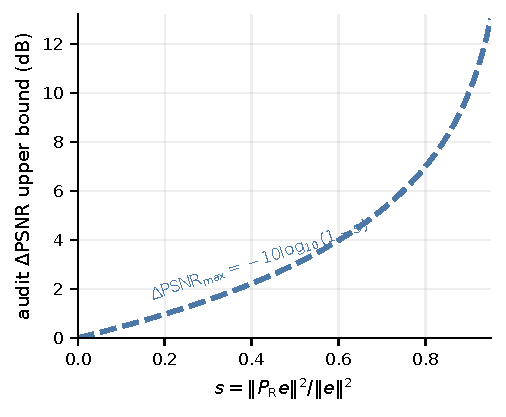
\includegraphics[width=\columnwidth]{figures/theorem2_psnr_bound.pdf}
    \caption{Theorem~1 hard-projection PSNR upper bound,
    $\Delta\mathrm{PSNR}_{\max}=-10\log_{10}(1-s)$, shown as a function of the
    pre-audit row-space error share $s$.  The measured flat-corner behavior of
    trained networks is reported numerically in Tables~\ref{tab:posthoc-audit}
    and~\ref{tab:ablation}: the audit moves PSNR by only $0.0136$ dB for Rad-5
    and $0.0387$ dB for Scr-5 while reducing measurement residuals by orders of
    magnitude.}
    \label{fig:flat-enhancement-corners}
\end{figure}

\subsection{Ablation Evidence}

Table~\ref{tab:ablation} reports the 5\% ablation rows.  Removing the final
audit or measurement loss leaves PSNR near the full learned output, but the
pre-audit measurement residual is much worse.  Applying the audit restores the
residual with little PSNR movement.  This is the empirical expression of
\eqref{eq:error-pythagoras}: image quality and measurement accountability are
coupled only through the row-space error share.

\begin{table*}[t]
\centering
\caption{Ablation and post-hoc audit rows.  PSNR changes are small, while
$\RelMeasErr$ changes by orders of magnitude, supporting the geometric
separation between image quality and measurement accountability.}
\label{tab:ablation}
\footnotesize
\resizebox{\textwidth}{!}{%
\begin{tabular}{lrrrrrr}
\toprule
Row & PSNR pre & PSNR post & $\Delta$PSNR & $\RelMeasErr$ pre & $\RelMeasErr$ post & contraction\\
\midrule
rad5\_no\_final\_audit & 22.192 & 22.206 & 0.0136 & \num{3.68e-2} & \num{1.90e-6} & \num{5.15e-5}\\
rad5\_no\_gate\_no\_final\_audit & 22.186 & 22.200 & 0.0136 & \num{3.69e-2} & \num{1.90e-6} & \num{5.15e-5}\\
rad5\_no\_final\_audit\_no\_meas\_loss & 22.180 & 22.219 & 0.0384 & \num{7.30e-2} & \num{3.76e-6} & \num{5.15e-5}\\
scr5\_no\_final\_audit & 22.146 & 22.185 & 0.0387 & \num{1.80e-2} & \num{1.80e-5} & \num{9.99e-4}\\
scr5\_no\_gate\_no\_final\_audit & 22.146 & 22.185 & 0.0385 & \num{1.80e-2} & \num{1.80e-5} & \num{9.99e-4}\\
scr5\_no\_final\_audit\_no\_meas\_loss & 22.138 & 22.171 & 0.0322 & \num{2.09e-2} & \num{2.09e-5} & \num{9.99e-4}\\
\bottomrule
\end{tabular}
}
\end{table*}

The Scr-5 ablation rows in Table~\ref{tab:ablation} are used only as audit
evidence; the Scr-5 GAN comparison metrics are reported separately in
Table~\ref{tab:scr5-canonical}.

\section{What the Certificate Cannot Do: The Verifiability Barrier}
\label{sec:limits}

The contraction certificate proves a statement about the measured component of an
image.  It does not prove that the unmeasured component is the one that would have
appeared in the scene.  This limitation is not a weakness of the particular
audit in Section~\ref{sec:audit}; it follows from the same range-null
decomposition that made the audit possible.

\subsection{A Feasible Wrong Image}

Let $x_i$ and $x_j$ be two images, and suppose that we want an image that has the
measurement of $x_i$ while retaining the null-space content of $x_j$.  Define
\begin{equation}
    u_{ij}
    =
    x_j - A^\pinv(Ax_j-y_i),
    \qquad y_i=Ax_i .
    \label{eq:feasible-hallucination}
\end{equation}
We now compute its measured component explicitly.  Since $y_i\in\range(A)$ and
$Ax_j\in\range(A)$, their difference $Ax_j-y_i$ lies in $\range(A)$.  The matrix
$AA^\pinv$ is the orthogonal projector onto $\range(A)$, so
\begin{align}
    Au_{ij}
    &= A x_j - AA^\pinv(Ax_j-y_i)                                      \\
    &= A x_j - (Ax_j-y_i)                                               \\
    &= y_i .                                                           
    \label{eq:feasible-hallucination-meas}
\end{align}
Thus $u_{ij}$ is perfectly measurement-consistent with the measurement of
$x_i$.  Its null-space component is
\begin{align}
    \PZ u_{ij}
    &= \PZ x_j - \PZ A^\pinv(Ax_j-y_i)                                  \\
    &= \PZ x_j ,
    \label{eq:feasible-hallucination-null}
\end{align}
The second equality holds because $\PZ A^\pinv=0$: $A^\pinv$ maps into the row
space and $\PZ$ annihilates that space.  Its row-space component is fixed by
$y_i$:
\begin{equation}
    \PR u_{ij}=A^\pinv Au_{ij}=A^\pinv y_i=\PR x_i .
    \label{eq:feasible-hallucination-row}
\end{equation}
In plain language, one can splice the measured part of one image to the
unmeasured part of another image and obtain a reconstruction that passes the
measurement audit exactly.

Table~\ref{tab:feasible-hallucination} reports the Rad-5 feasible-pair
construction.  The constructed wrong images have residuals at floating-point
scale while remaining visually wrong with respect to the target image.  These
rows are the cleanest empirical reminder that consistency is not truth.

\begin{table}[t]
\centering
\caption{Feasible wrong-image construction for Rad-5.  The constructed image
$u_{ij}$ is measurement-consistent with $y_i$ but keeps $\PZ x_j$.  Therefore a
small residual certifies the measured component, not semantic correctness.}
\label{tab:feasible-hallucination}
\footnotesize
\resizebox{\columnwidth}{!}{%
\begin{tabular}{lrrrr}
\toprule
Family & pairs & $\RelMeasErr(u_{ij},y_i)$ & truth residual & PSNR$(u_{ij},x_i)$\\
\midrule
Rad-5 & 8 & \num{2.16e-15}\,--\,\num{4.00e-15} &
\num{3.45e-3}\,--\,\num{7.46e-3} &
7.697--11.378\\
\bottomrule
\end{tabular}
}
\end{table}

\begin{figure}[t]
    \centering
    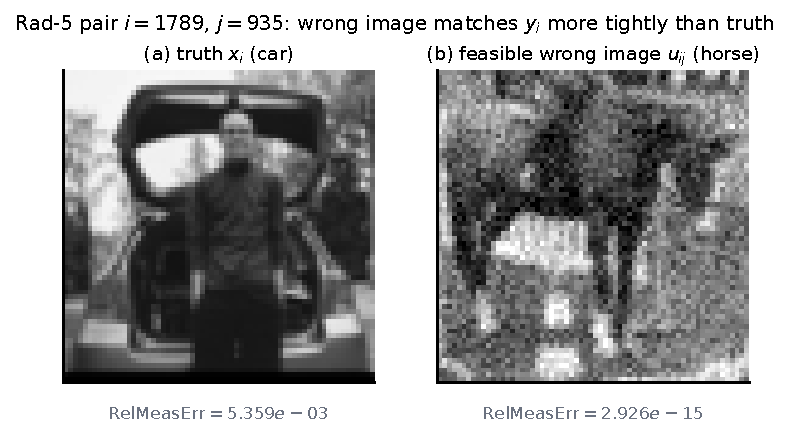
\includegraphics[width=\columnwidth]{figures/feasible_hallucination_pair.pdf}
    \caption{Feasible hallucination for a Rad-5 feasible-pair output
    ($i=1789$, $j=935$).  The true target image is a car with
    $\RelMeasErr(x_i,y_i)=\num{5.36e-3}$, while the constructed wrong image
    $u_{ij}=x_j-A^\dagger(Ax_j-y_i)$ visually follows the horse donor and has
    $\RelMeasErr(u_{ij},y_i)=\num{2.93e-15}$.  Thus an image can satisfy
    the measurement record more tightly than the noisy truth while remaining
    semantically wrong.}
    \label{fig:feasible-hallucination}
\end{figure}

\subsection{Magnitude Is Not Pixelwise Correctness}

The previous construction shows that an audit cannot identify the correct
null-space image.  A second, more operational question is whether the observable
map $|\PZ\hat{x}|$ can be used as a pixelwise error map.  We call it a
prior-supplied-content map: it shows where the prior supplied null-space
content, not where the reconstruction is wrong.  The
range-null decomposition again gives the relevant algebra.  Let
$\hat{x}$ be any audited reconstruction.  Then the null-space error is
\begin{equation}
    \PZ(\hat{x}-x)=\PZ\hat{x}-\PZ x .
    \label{eq:p0-error}
\end{equation}
The observable magnitude $|\PZ\hat{x}|$ contains no direct term for the unknown
$\PZ x$; it is a property of the reconstruction, not an error certificate.  A
large value in the prior-supplied-content map may be accurate texture,
inaccurate texture, or a harmless choice among feasible completions.  Magnitude
does not indicate correctness.

Table~\ref{tab:p0-map} reports the $96\times96$ Rad-5 validation.
For the learned arms B and C, the pixels with the largest $|\PZ\hat{x}|$ do not
have larger actual null-space error; the top-10\% error is lower than the
remaining 90\%.  The negative result is the point: null-space magnitude and
null-space correctness are empirically decoupled.

\begin{table}[t]
\centering
\caption{The prior-supplied-content map $|\PZ\hat{x}|$ is not a pixelwise error
map on the $96\times96$ Rad-5 validation.  Spearman and Pearson correlations
are near zero.  For arms B and C, the top-10\% $|\PZ\hat{x}|$ pixels have lower
actual $\PZ$ error than the remaining pixels.}
\label{tab:p0-map}
\footnotesize
\resizebox{\columnwidth}{!}{%
\begin{tabular}{lrrrr}
\toprule
Arm & Spearman & Pearson & top-10\% error & rest-90\% error\\
\midrule
A & -0.079 & -0.069 & 0.259 & 0.242\\
B &  0.073 &  0.061 & 0.071 & 0.079\\
C &  0.072 &  0.061 & 0.071 & 0.079\\
\bottomrule
\end{tabular}
}
\end{table}

\subsection{Amount, Distribution, and Correctness Are Separate}

Posterior sampling makes the boundary sharper.  For a fixed $y$, a sampler
returns $\hat{x}^{(k)}=\Audit(v^{(k)})$.  By Section~\ref{sec:audit},
$A\hat{x}^{(k)}\approx y$ for every $k$ when $\lambda$ is small.  However, the
sample variance splits as
\begin{align}
    \mathrm{Var}(\hat{x}^{(k)})
    &=
    \mathrm{Var}(\PR\hat{x}^{(k)}+\PZ\hat{x}^{(k)})                    \\
    &=
    \mathrm{Var}(\PR\hat{x}^{(k)})
    +
    \mathrm{Var}(\PZ\hat{x}^{(k)}),
    \label{eq:variance-split}
\end{align}
where the cross term vanishes because $\PR$ and $\PZ$ project onto orthogonal
subspaces.  The audit can drive the first term to the measurement noise floor,
but it says neither how large the second term should be nor whether its mean is
centered on the true $\PZ x$.  Thus the amount of uncertainty, the distribution
of samples, and the correctness of the unmeasured content are three different
questions.

Table~\ref{tab:posterior-calibration} summarizes the posterior-calibration
diagnostics, with the full gate-by-gate table in
Appendix~\ref{app:posterior-diagnostics}.  A deterministic Rad-5 checkpoint collapses at
the $10^{-3}$ pixel-std scale and $10^{-6}$ $\PZ$-variance scale.  Replacing
full reconstruction loss with row-space-only reconstruction restores null-space
variation to the $10^{-2}$ pixel-std scale and $10^{-3}$ $\PZ$-variance scale.
The restored variation is not merely white noise: the spectral sanity gate
passes a non-white, low-frequency-structured check.  The standard deviations,
variances, slope, and high-to-low ratio are summarized in
Table~\ref{tab:posterior-calibration} and reported gate-by-gate in
Table~\ref{tab:posterior-calibration-full}.  In plain language, the collapse was not
an architectural dead end; the full reconstruction loss was suppressing
feasible null-space diversity, and removing that pressure lets structured null
variation appear.

Calibration remains unresolved for a different reason.  The uncentered
calibration audit has
subnominal 90\% coverage and a nonzero $\PZ$ mean offset: pairwise diversity can
increase spread while leaving the sample cloud centered in the wrong place.
Adding a $\PZ$ mean anchor improves the center but collapses the spread; the
best anchor/diversity scan still reaches only about 45\% pixel coverage and
48\% $\PZ$ coverage at the nominal 90\% level.  The results identify the
base bottleneck: the deterministic base estimate has $\PZ$ det-to-GT RMSE about
0.081, while the best scan has $\PZ$ mean-to-GT RMSE about 0.088.  Exact
coverage, offset, and RMSE values are summarized in
Table~\ref{tab:posterior-calibration} and fully listed in
Table~\ref{tab:posterior-calibration-full}.
Plainly, a sampler can learn to move inside the null-space affine set, but if
the base reconstruction is centered on the wrong $\PZ$ content, spread tuning
alone cannot make the posterior calibrated.

\begin{table*}[t]
\centering
\caption{Posterior-sampling diagnostic summary.  The row-space-only diagnostic
restores $\PZ$ variation while preserving measurement consistency, but the
anchor/diversity scan remains under-calibrated and the base $\PZ$ estimate is
offset from ground truth.  Full gate-by-gate diagnostics are in
Table~\ref{tab:posterior-calibration-full}.}
\label{tab:posterior-calibration}
\footnotesize
\resizebox{\textwidth}{!}{%
\begin{tabular}{llrrr@{\hspace{1.0em}}l}
\toprule
Gate & diagnostic & fixed-$y$ std & $\PZ$ var & max $\RelMeasErr$ & key posterior evidence\\
\midrule
1 & deterministic Rad-5 baseline &
0.0010 & \num{1.09e-6} &
\num{3.84e-5} & collapse\\
2 & row-space-only reconstruction &
0.0335 & \num{1.28e-3} &
\num{5.61e-5} & anti-collapse pass\\
6 & anchor/diversity scan &
0.0349 & \num{1.39e-3} &
\num{5.62e-5} & 90\% pixel/$\PZ$ cov. 0.453 / 0.478; offset 0.0331\\
7 & base $\PZ$ bottleneck &
n.r. & n.r. & n.r. & det-to-GT RMSE 0.0810; best mean-to-GT RMSE 0.0877\\
\bottomrule
\end{tabular}
}
\end{table*}

The gate-by-gate coverage diagnostics are reported in
Table~\ref{tab:posterior-calibration-full}; no separate coverage-evolution figure is
needed for this evidence.

\subsection{Operator Drift Is Visible to the Certificate}

The measurement certificate is also useful when the deployed operator is not the
operator assumed by the audit.  We include a simulation-scoped
operator-drift experiment: the audit is performed with a drifted operator, and
the residual is then evaluated against the original true operator.  This is not
a hardware-robustness claim.  It is a calibration-mismatch probe inside the
simulation setup.

Table~\ref{tab:adrift} shows the pattern.  For Rad-5, increasing the relative
operator drift from $0$ to $0.05$ changes post-audit PSNR only from 22.206 dB
to 22.178 dB, while the residual against the true operator rises from
\num{1.90e-6} to \num{4.88e-2}.  For Scr-5, the same drift
range changes PSNR from 22.185 dB to 22.155 dB, while the true-operator
residual rises from \num{1.80e-5} to \num{1.26e-2}.  In
plain language, PSNR barely sees the calibration mismatch, while the certificate
does.

\begin{table}[t]
\centering
\caption{Simulation-scoped operator-drift probe.  The audit uses a drifted
operator, while $\RelMeasErr$ is evaluated against the true operator.  PSNR is
nearly flat, but the certificate residual rises by orders of magnitude.}
\label{tab:adrift}
\footnotesize
\resizebox{\columnwidth}{!}{%
\begin{tabular}{lrr@{\hspace{0.8em}}r}
\toprule
Regime & drift & post $\RelMeasErr$ true $A$ & post PSNR\\
\midrule
Rad-5 & 0.000 & \num{1.90e-6} & 22.206\\
Rad-5 & 0.005 & \num{4.89e-3} & 22.206\\
Rad-5 & 0.010 & \num{9.79e-3} & 22.205\\
Rad-5 & 0.020 & \num{1.96e-2} & 22.201\\
Rad-5 & 0.050 & \num{4.88e-2} & 22.178\\
Scr-5 & 0.000 & \num{1.80e-5} & 22.185\\
Scr-5 & 0.005 & \num{1.26e-3} & 22.184\\
Scr-5 & 0.010 & \num{2.53e-3} & 22.183\\
Scr-5 & 0.020 & \num{5.06e-3} & 22.180\\
Scr-5 & 0.050 & \num{1.26e-2} & 22.155\\
\bottomrule
\end{tabular}
}
\end{table}

\subsection{Wrong Measurements Break the Reconstruction}

A separate dependence test asks whether the learned reconstructor uses the
recorded measurement or merely emits plausible samples from the data prior.  The
experiment perturbs the measurement input in two ways: by rolling the
batch so that each image receives another image's $y$, and by shuffling the
measurement coordinates.  Table~\ref{tab:wrong-y} reports 500-image probes.
Across Rad-5, Scr-5, Rad-10, and Scr-10, wrong-$y$ inputs reduce PSNR by
12.174--14.793 dB, and shuffled-$y$ inputs reduce PSNR by 14.537--17.026
dB.  In plain language, the model is not acting as a pure dataset prior; it
depends strongly on the recorded measurement.

This dependence does not contradict the range-null geometry in
Section~\ref{sec:quality-accountability}.  The linear operator $A$
geometrically constrains only the row-space component: every feasible image may
still differ by an arbitrary $\PZ$ component.  A trained conditional
reconstructor is a different object: it uses $y$ as an input to choose which
prior-supplied $\PZ$ completion to emit.  Thus the wrong-$y$ collapse shows that
the network really conditions its null-space completion on the recorded
measurement; it does not mean that the measurement geometry itself constrains
the null space.

\begin{table}[t]
\centering
\caption{Wrong-measurement dependence test.  Replacing the measurement record by
another sample's $y$ or shuffling measurement coordinates causes large PSNR
drops, showing that the reconstructor uses the recorded measurement.}
\label{tab:wrong-y}
\footnotesize
\resizebox{\columnwidth}{!}{%
\begin{tabular}{lrrrrr}
\toprule
Model & clean & wrong-$y$ & drop & shuffled-$y$ & drop\\
\midrule
main\_rad5 & 22.202 & 9.962 & 12.241 & 7.481 & 14.721\\
main\_scr5 & 22.160 & 9.986 & 12.174 & 7.624 & 14.537\\
main\_rad10 & 24.678 & 9.886 & 14.793 & 7.652 & 17.026\\
main\_scr10 & 24.604 & 9.887 & 14.717 & 7.597 & 17.007\\
\bottomrule
\end{tabular}
}
\end{table}

\subsection{The Unified Boundary}

The three verifiability-barrier tests in Sections~V-A--V-C are one
theorem-shaped message.  Equation
\eqref{eq:feasible-hallucination-null} shows that null-space correctness cannot
be certified by $A\hat{x}=y$.  Equation \eqref{eq:p0-error} shows that
null-space magnitude is not an error map because the unknown term $\PZ x$
remains absent.  Equation \eqref{eq:variance-split} shows that sample diversity
can be created in $\PZ$ while its center and coverage remain wrong.  In plain
language, the amount of unmeasured content, the distribution of unmeasured
content, and the correctness of unmeasured content are decoupled.

This is the verifiability barrier.  The certificate guarantees row-space
accountability: the reconstruction agrees with the measurement-supported
component up to the contraction/noise floor.  It cannot verify the correctness
of prior-supplied $\PZ$ content, and the experiments show that two tempting
workarounds also fail: $|\PZ\hat{x}|$ does not localize error, and learned
measurement-consistent sampling does not automatically calibrate the posterior.
These are not separate disappointments.  Section~V-B is the single-reconstruction
face of the barrier: after seeing one audited image, the magnitude of
$\PZ\hat{x}$ does not reveal where $\PZ\hat{x}-\PZ x$ is large.  Section~V-C is
the sampling face of the same barrier: even a cloud of measurement-consistent
samples remains limited by the base estimator's $\PZ$ bias, because the
measurement provides no corrective signal for that bias.  The obstruction in
both cases is exactly $A\PZ=0$.

\section{A Generative Prior Under the Certificate: GAN as a Case Study}
\label{sec:gan}

We use a GAN branch as a controlled example of a learned prior operating inside
the range-null geometry.  The GAN is not the main claim of this paper, and we do
not claim state-of-the-art perceptual quality or superiority over diffusion
models.  The purpose is narrower: to show how a generative prior can change
audited null-space content while the measurement certificate remains attached to
the output.

\subsection{Gauge-Equalized Discrimination}

An unconditional discriminator can learn shortcuts in the measured component.  A
range-null reading makes this failure mode explicit.  If the discriminator sees
$\PR\hat{x}$ differences caused by measurement residual, it may reward or punish
measurement artifacts instead of image prior structure.  The gauge-equalized
branch is designed to reduce this shortcut by focusing the adversarial signal on
content that is not already certified by the measurement audit.

The diagnostic results support the presence of such signal.  Table
\ref{tab:gauge-regime} summarizes the Scr-5 gauge AUCs and the regime
map: the patch-GAN unconditional gauge is about 0.85 AUC, the conditional
image-data gauge is about 0.73 AUC, and the residual-feature logistic diagnostic
is about 0.98 AUC.  Scr-5 and Rad-5 pass the train/evidence gate, while Scr-10
and Rad-10 are weak-gate regimes where the GAN branch is not advanced.

\begin{table}[t]
\centering
\caption{Gauge diagnostics and regime gating.  The GAN branch is used only where
the diagnostic signal is present; weak-gate 10\% regimes are stopped rather than
used for a quality claim.}
\label{tab:gauge-regime}
\footnotesize
\resizebox{\columnwidth}{!}{%
\begin{tabular}{lrrl}
\toprule
Regime/diagnostic & AUC & CI/source & decision\\
\midrule
Scr-5 patch-GAN unconditional gauge & 0.847 & 0.824--0.874 & positive\\
Scr-5 conditional image-data gauge & 0.731 & 0.696--0.758 & positive\\
Scr-5 residual-feature logistic & 0.980 & 0.967--0.990 & positive\\
Rad-5 regime map & 0.877 & 0.845--0.907 & train/evidence positive\\
Scr-10 regime map & 0.624 & 0.579--0.670 & weak gate; stop\\
Rad-10 regime map & 0.640 & 0.590--0.677 & weak gate; stop\\
\bottomrule
\end{tabular}
}
\end{table}

The shortcut stress test in Table~\ref{tab:shortcut} shows why the distinction
matters.  At $\alpha=0.1$, row-space perturbations produce a standard
discriminator fake-score delta of about 0.477, whereas the gauge-discriminator
row delta is 0.  Null-space perturbations produce a gauge-discriminator delta
of about 0.739.  This is the desired direction for a prior module: the
adversarial signal should not be a surrogate measurement-residual detector.

\begin{table}[t]
\centering
\caption{Shortcut stress test at $\alpha=0.1$.  The gauge discriminator is
insensitive to row-space perturbations and responds to null-space perturbations,
which aligns the prior signal with the unmeasured component.}
\label{tab:shortcut}
\footnotesize
\resizebox{\columnwidth}{!}{%
\begin{tabular}{lllr@{\hspace{0.8em}}r}
\toprule
Model & base & perturbation & delta & mean $\RelMeasErr$\\
\midrule
standard D & real & row & 0.384 & \num{1.13e-1}\\
standard D & real & null & 0.401 & \num{5.55e-3}\\
standard D & fake mean & row & 0.477 & \num{1.12e-1}\\
standard D & fake mean & null & 0.485 & \num{5.58e-3}\\
gauge D & real & row & 0.000 & \num{1.13e-1}\\
gauge D & real & null & 0.540 & \num{5.55e-3}\\
gauge D & fake mean & row & 0.000 & \num{1.12e-1}\\
gauge D & fake mean & null & 0.739 & \num{5.58e-3}\\
\bottomrule
\end{tabular}
}
\end{table}

\subsection{Controlled $96\times96$ Rad-5 Result}

Table~\ref{tab:task2-rad5} reports the controlled $96\times96$ Rad-5 GAN
paired-seed comparison over ten seeds.  The gauge branch C improves LPIPS and
RAPSD relative to the baseline branch B with the same sign in all ten paired
seeds: mean C--B LPIPS is $-0.00552$ and mean C--B RAPSD is
$-\num{7.48e-4}$.  The within-seed per-sample bootstrap intervals exclude zero,
and the ten-seed sign consistency is substantially stronger than the earlier
three-seed probe.

The ten-seed PSNR result is also sign-consistent, but its interpretation is
different.  C--B PSNR is positive in 10/10 seeds with seed-level mean
$+0.0148$ dB, a $t$ 95\% confidence interval of $[+0.0107,+0.0189]$ dB, and a
bootstrap 95\% confidence interval of $[+0.0113,+0.0180]$ dB.  Because B and C
are identical except for the gauge adversarial branch, that branch is the source
of this displacement.  The observation is consistent with the soft-audit
framework: under a hard projection ($\lambda\to0$), the row-space component of
both branches would be pinned by the measurement, whereas the soft audit
($\lambda>0$) leaves a small margin in which the branches can differ slightly.
We do not localize this gain to a specific component, row-space or null-space.
The gain is at the $0.01$--$0.02$ dB level and is not a quality claim; the
perceptual/spectral improvements and the unchanged certificate remain the
point.  B and C remain measurement accountable: the seed-mean $\RelMeasErr$
averages are \num{9.28e-5} and \num{9.90e-5}, respectively, and the B/C
per-sample maximum is \num{1.61e-4}.

\begin{table}[t]
\centering
\caption{$96\times96$ Rad-5 controlled GAN, ten paired seeds.  C--B is negative
for LPIPS and RAPSD in all ten seeds, while C--B PSNR is a real but tiny
positive shift under the soft audit.  Rad-5 $\RelMeasErr$ stays on the audited
$10^{-4}$ scale.}
\label{tab:task2-rad5}
\footnotesize
\resizebox{\columnwidth}{!}{%
\begin{tabular}{lccc}
\toprule
Quantity & sign consistency & mean C--B / value & 95\% CI or support\\
\midrule
LPIPS & 10/10 negative & $-0.00552$ & per-sample bootstrap excludes 0\\
RAPSD & 10/10 negative & $-\num{7.48e-4}$ & per-sample bootstrap excludes 0\\
PSNR & 10/10 positive & $+0.0148$ dB & $t$: $[+0.0107,+0.0189]$ dB; boot: $[+0.0113,+0.0180]$ dB\\
$\RelMeasErr$ & -- & B: \num{9.28e-5}; C: \num{9.90e-5} & B/C per-sample max: \num{1.61e-4}\\
\bottomrule
\end{tabular}
}
\end{table}

\subsection{Standard cGAN Control}

A fair reading also requires a standard cGAN control.  Table~\ref{tab:standard}
shows the $96\times96$ Rad-5 standard-control focus metrics.  The standard branch D and
the gauge branch C are comparable and mixed: the seed-level wins go in both
directions and the magnitudes are small.  This prevents the GAN section from
becoming a dominance claim.

The small effect size is also geometrically expected.  For two audited
reconstructions of the same measurement, $\hat{x}_1$ and $\hat{x}_2$, hard
consistency would give $\PR\hat{x}_1=\PR\hat{x}_2=A^\pinv y$, and soft
consistency makes this equality approximate.  Their difference is therefore
mostly null-space:
\begin{equation}
    \hat{x}_1-\hat{x}_2
    =
    \PR(\hat{x}_1-\hat{x}_2)+\PZ(\hat{x}_1-\hat{x}_2)
    \approx
    \PZ(\hat{x}_1-\hat{x}_2).
    \label{eq:gan-null-delta}
\end{equation}
For a fixed ground truth $x$, write $e_i=\hat{x}_i-x$.  The squared error
changes as
\begin{align}
    \|e_2\|_2^2-\|e_1\|_2^2
    &=
    \|\PR e_2\|_2^2-\|\PR e_1\|_2^2        \\
    &\quad+
    \|\PZ e_2\|_2^2-\|\PZ e_1\|_2^2 .
    \label{eq:gan-psnr-null}
\end{align}
The first difference is small after auditing, so any perceptual improvement
from the GAN prior must come mostly from changing $\PZ$ content.  Plainly, the
prior can make the null-space content look more natural without guaranteeing a
lower Euclidean distance to the hidden true $\PZ x$; that is why LPIPS/RAPSD can
move while PSNR barely moves.

\begin{table*}[!t]
\centering
\caption{$96\times96$ Rad-5 standard cGAN control.  D--C differences are mixed across
seeds and metrics, supporting the limited claim that the gauge branch is a
controlled prior example rather than a universal improvement over a standard
cGAN.}
\label{tab:standard}
\footnotesize
\begin{tabular}{llrrr}
\toprule
Seed & metric & C & D\_standard & D--C\\
\midrule
1 & PSNR & 19.789 & 19.788 & -0.0017\\
1 & SSIM & 0.458 & 0.458 & -0.0001\\
1 & RAPSD & 0.0089 & 0.0089 & 0.0000\\
1 & LPIPS & 0.411 & 0.411 & 0.0002\\
2 & PSNR & 19.788 & 19.788 & 0.0008\\
2 & SSIM & 0.458 & 0.459 & 0.0004\\
2 & RAPSD & 0.0089 & 0.0089 & 0.0000\\
2 & LPIPS & 0.415 & 0.415 & 0.0000\\
3 & PSNR & 19.788 & 19.788 & -0.0004\\
3 & SSIM & 0.459 & 0.459 & 0.0000\\
3 & RAPSD & 0.0087 & 0.0087 & 0.0000\\
3 & LPIPS & 0.413 & 0.413 & 0.0000\\
\bottomrule
\end{tabular}
\end{table*}

\subsection{Controlled Scr-5 Metrics}

Because several Scr-5 training protocols were evaluated during development,
Table~\ref{tab:scr5-canonical} is the only table in this section that reports
Scr-5 PSNR, SSIM, LPIPS, RAPSD, and $\RelMeasErr$ values for the GAN comparison.
The section does not mix Scr-5 metrics across protocol variants.

\begin{table*}[t]
\centering
\caption{Controlled Scr-5 5\% metrics.  These are the only Scr-5 GAN-branch
quality/accountability metrics used in Section~\ref{sec:gan}.
For this Scr-5 regime the audited $\RelMeasErr$ values are on the $10^{-3}$
scale, unlike the Rad-5 $96\times96$ rows in Table~\ref{tab:task2-rad5}.}
\label{tab:scr5-canonical}
\footnotesize
\begin{tabular}{lrrrr@{\hspace{0.8em}}r}
\toprule
Arm & PSNR & SSIM & LPIPS & RAPSD & $\RelMeasErr$\\
\midrule
B & 22.262 & 0.627 & 0.2349 & 0.0054 & \num{5.56e-3}\\
C\_gauge & 22.257 & 0.628 & 0.2308 & 0.0052 & \num{5.57e-3}\\
D\_standard & 22.258 & 0.628 & 0.2310 & 0.0052 & \num{5.57e-3}\\
\bottomrule
\end{tabular}
\end{table*}

\section{Related Work}
\label{sec:related}

\subsection{Range-Null Diffusion and DDNM-Style Solvers}

Range-null diffusion and DDNM-style inverse solvers also use a decomposition of
measured and unmeasured components [CITE].  The delta here is the certification
question: we use the decomposition to define a test-time measurement audit, to
prove its contraction certificate, and to state what the certificate cannot
verify.  The GAN branch also introduces a discriminator-shortcut issue that is
orthogonal to diffusion sampling: an adversarial discriminator can learn row
residual shortcuts unless its input is gauge-equalized.

\subsection{Adversarial Regularization}

Adversarial regularizers have long been used to make inverse-problem outputs
look more natural [CITE].  Our distinction is that the prior is placed under a
measurement certificate.  The discriminator is not treated as a quality oracle:
it is audited for shortcut sensitivity, and its effect is interpreted as
prior-supplied $\PZ$ content rather than certified truth.

\subsection{Deep Null-Space Learning}

Deep null-space learning explicitly trains networks to fill the null component
of an inverse problem [CITE].  In the notation of this paper, the supervised
null-space arm B is a representative of that idea.  We add a soft,
noise-aware certificate $\Audit$, and we analyze the verifiability of the
learned $\PZ$ content itself.  The negative map and posterior-calibration
results show that producing a plausible null-space estimate is different from
certifying where it is wrong or calibrating its distribution.

\subsection{Data Consistency and Projection Layers}

Projection and data-consistency layers enforce agreement with the measurement
operator in many reconstruction networks [CITE].  Our audit
$\Audit(v)=v-\Blambda(Av-y)$ can be read as a soft data-consistency layer, but
the contribution is semantic and geometric: we derive its singular-mode
contraction, separate its PSNR effect from its accountability effect, and state
the feasible-hallucination boundary that no projection layer can cross.

\subsection{Diffusion Inverse Solvers}

DPS, DDRM, $\Pi$GDM, and related diffusion inverse solvers are important
quality baselines [CITE].  We do not claim to beat them.  Our claim is about
certification and verifiability rather than state-of-the-art reconstruction:
even a stronger sampler can only be certified in $\PR$ by the measurement, while
its $\PZ$ center, spread, and correctness must be evaluated separately.  In
plain language, better generative modeling may improve the prior-supplied
content, but it does not erase the range-null boundary.

\section{Discussion and Conclusion}
\label{sec:conclusion}

The main message of this paper is that under-sampled ghost imaging has a
two-part geometry.  The row-space component $\PR x=A^\pinv Ax$ is the part the
measurement can see, and the null-space component $\PZ x=(I-A^\pinv A)x$ is the
part the measurement cannot see.  Once this split is made explicit, several
observations that can look empirical become the same mathematical fact.  The
audit in Section~\ref{sec:audit} contracts measurement residuals because it acts
on the row-space residual.  The PSNR response in Section~\ref{sec:quality-accountability}
is small for trained networks because their remaining error is mostly outside
the row-space share that the audit can change.  The feasible hallucinations and
posterior-calibration failures in Section~\ref{sec:limits} persist because the
measurement cannot identify the correct $\PZ x$.

The practical recommendation is therefore not to replace image-quality metrics
with measurement residuals, nor to replace measurement residuals with image
metrics.  They answer different questions.  PSNR, SSIM, LPIPS, RAPSD, and
related metrics evaluate agreement with a reference or perceptual proxy when
such a reference is available.  The audit evaluates whether the reported image
is accountable to the measurement available at deployment time.  A trustworthy
pipeline should report both, and should state clearly which part of the image is
measured, which part is prior-supplied, and which claims cannot be verified
without ground truth.

A natural concern is whether enforcing measurement consistency degrades the
naturalness of the reconstruction relative to an unconstrained end-to-end
network.  In our pipeline this is not the case for a structural reason: the
reconstruction loss is applied to the final projected output
$\hat{x}=\Audit(\cdot)$ rather than to the null-space residual in isolation, and
the projection is part of the forward pass during training.  The network is
therefore trained end-to-end through the range-null projection, learning to
produce a natural full image under the constraint that its row-space component is
locked to $A^\pinv y$.  Empirically the cost of the projection is negligible:
the audit moves PSNR by less than $0.04$ dB
(Tables~\ref{tab:posthoc-audit} and~\ref{tab:ablation}) while the audited
reconstructions retain strong perceptual quality (LPIPS/RAPSD,
Section~\ref{sec:gan}).  Naturalness is supplied by the trained prior and
measurement consistency is guaranteed by the audit; because the prior is trained
under the audit, the two are obtained jointly rather than traded off.  We
emphasize, however, that the audit itself does not enforce naturalness: a
measurement-consistent reconstruction can be unnatural, as in the constructed
$u_{ij}$ in Fig.~\ref{fig:pipeline-range-null}, which is precisely the
measurement-consistency $\ne$ correctness $\ne$ naturalness distinction.

There are important limitations.  The experiments in this manuscript are
simulation-based; hardware ghost-imaging validation is left to future work.  The
posterior-sampling line shows restored null-space diversity but not calibrated
coverage.  The GAN branch gives a controlled example of a prior under audit, not
a claim that GANs are the best generative model for this problem; its effect is
small and comparable to a standard cGAN control.  The experimental scope is one
ghost-imaging problem.  The range-null principle applies to general linear
inverse problems, but cross-domain validation is outside the scope of this
study; any inpainting or toy feasibility example should be read only as
feasibility evidence, not as a deployment claim.  Diffusion, flow, and
score-based priors should be evaluated under the same range-null audit and the
same negative tests [CITE].  Finally, the posterior-calibration results indicate
that sampling quality is bounded by the base estimator's null-space accuracy,
not only by the diversity mechanism.

In conclusion, range-null separability gives a compact language for measured and
unmeasured content in ghost imaging.  It enables a plug-in, test-time,
ground-truth-free certificate of measurement consistency, explains when that
certificate can or cannot improve image quality, and exposes the fundamental
boundary of verification: consistency is certifiable, but the correctness of
prior-supplied null-space content is not certified by the measurement alone.

\appendices

\refstepcounter{section}
\section*{Appendix \thesection: Full Posterior-Sampling Diagnostics}
\label{app:posterior-diagnostics}

Table~\ref{tab:posterior-calibration-full} gives the full gate-by-gate
posterior-sampling diagnostics summarized in
Table~\ref{tab:posterior-calibration}.

\begin{table*}[t]
\centering
\caption{Full posterior-sampling diagnostics.  The row-space-only diagnostic
restores $\PZ$ variation while preserving measurement consistency, but coverage
remains under-calibrated.  Entries marked n.r. were not recorded for that gate
or are not applicable to the calibration/bottleneck diagnostic represented by
the row.}
\label{tab:posterior-calibration-full}
\footnotesize
\resizebox{\textwidth}{!}{%
\begin{tabular}{llrrr@{\hspace{1.0em}}l}
\toprule
Gate & diagnostic & fixed-$y$ std & $\PZ$ var & max $\RelMeasErr$ & reported status\\
\midrule
1 & deterministic Rad-5 baseline &
0.0010 & \num{1.09e-6} &
\num{3.84e-5} & collapse\\
2 & row-space-only reconstruction &
0.0335 & \num{1.28e-3} &
\num{5.61e-5} & anti-collapse pass\\
3 & spectral sanity &
0.0335 & \num{1.28e-3} &
\num{5.61e-5} & slope -2.62; high/low \num{5.37e-3}\\
4 & uncentered calibration audit &
n.r. & n.r. & n.r. & 90\% pixel/$\PZ$ cov. 0.381 / 0.407; offset 0.0549\\
5 & centered diversity &
0.0069 & \num{5.19e-5} &
\num{4.63e-5} & 90\% pixel/$\PZ$ cov. 0.106 / 0.102; offset 0.0180\\
6 & anchor/diversity scan &
0.0349 & \num{1.39e-3} &
\num{5.62e-5} & 90\% pixel/$\PZ$ cov. 0.453 / 0.478; offset 0.0331\\
7 & base $\PZ$ bottleneck &
n.r. & n.r. & n.r. & det-to-GT RMSE 0.0810; best mean-to-GT RMSE 0.0877\\
\bottomrule
\end{tabular}
}
\end{table*}

\end{document}
